\chapter{Human Driver Modelling}

In this chapter, the human driver model that Salvucci presents in \cite{salvucci_1} is implemented and the metrics used to verify the model are established. Initially, the model is implemented in \textit{Matlab} using the continuous driver model. To be able to verify it using the probabilistic model checking techniques presented in Chapter 2, the model undergoes an abstraction process, out of which a discrete-time Markov chain is obtained using several different approaches and assumptions. Metrics are then established to be able to evaluate whether the model meets the requirements and how well the human performs in a given situation. Finally, a simulator is presented in Section~\ref{sec:simulator} in order to allow visualisation of paths in the model.

\section{Continuous Driver Model using ACT-R}

In order to obtain a continuous driver model, we interpret Salvucci's integrated driver model as presented in \cite{salvucci_1}. The scenario considered is the one Salvucci envisioned: a multilane highway with moderate (or low) traffic \cite{salvucci_1}. The model uses the three modules presented in Figure~\ref{fig:high_level_salvucci}, that is, monitoring, decision making and control. All these modules rely on the constant update of the environment, as some are based on visual perception or low-level perception cues. While the human model is presented clearly in \cite{salvucci_1}, the dynamics of the car (which is part of the environment) are left to the reader, as it is outside the scope of the paper. In that sense, some assumptions had to be made about the environment.

The main initial assumption is that the driver is perfectly aware of its surroundings, and thus it is able to obtain the positions of other vehicles (within a certain distance) and the near and far points perfectly (this assumption is challenged later in the abstraction process). It is also assumed that the vehicle the driver is using is directly controlled by the updating of any pertinent variables within the control module of the architecture (i.e. there is no intermediate system or separation). The environment is assumed to change at the same rate as a cycle of the ACT-R model.

The overall view of the system is presented in Figure~\ref{fig:driver_model_overview}. The information flow is marked using the dotted arrows, while the sequential flow of the program is marked in the filled, lighter gray ones. Both the monitoring and the decision making make use of the perception which corresponds to querying the environment for the information (e.g. near and far point or another vehicle's position). The control both queries and sends updated information (e.g. vehicle position) to the environment. Modules are updated sequentially, following the order: control, monitoring, decision making and environment (e.g. position, velocity and acceleration of other vehicles).

\vspace{1em}
\begin{figure}[h]
    \centering
    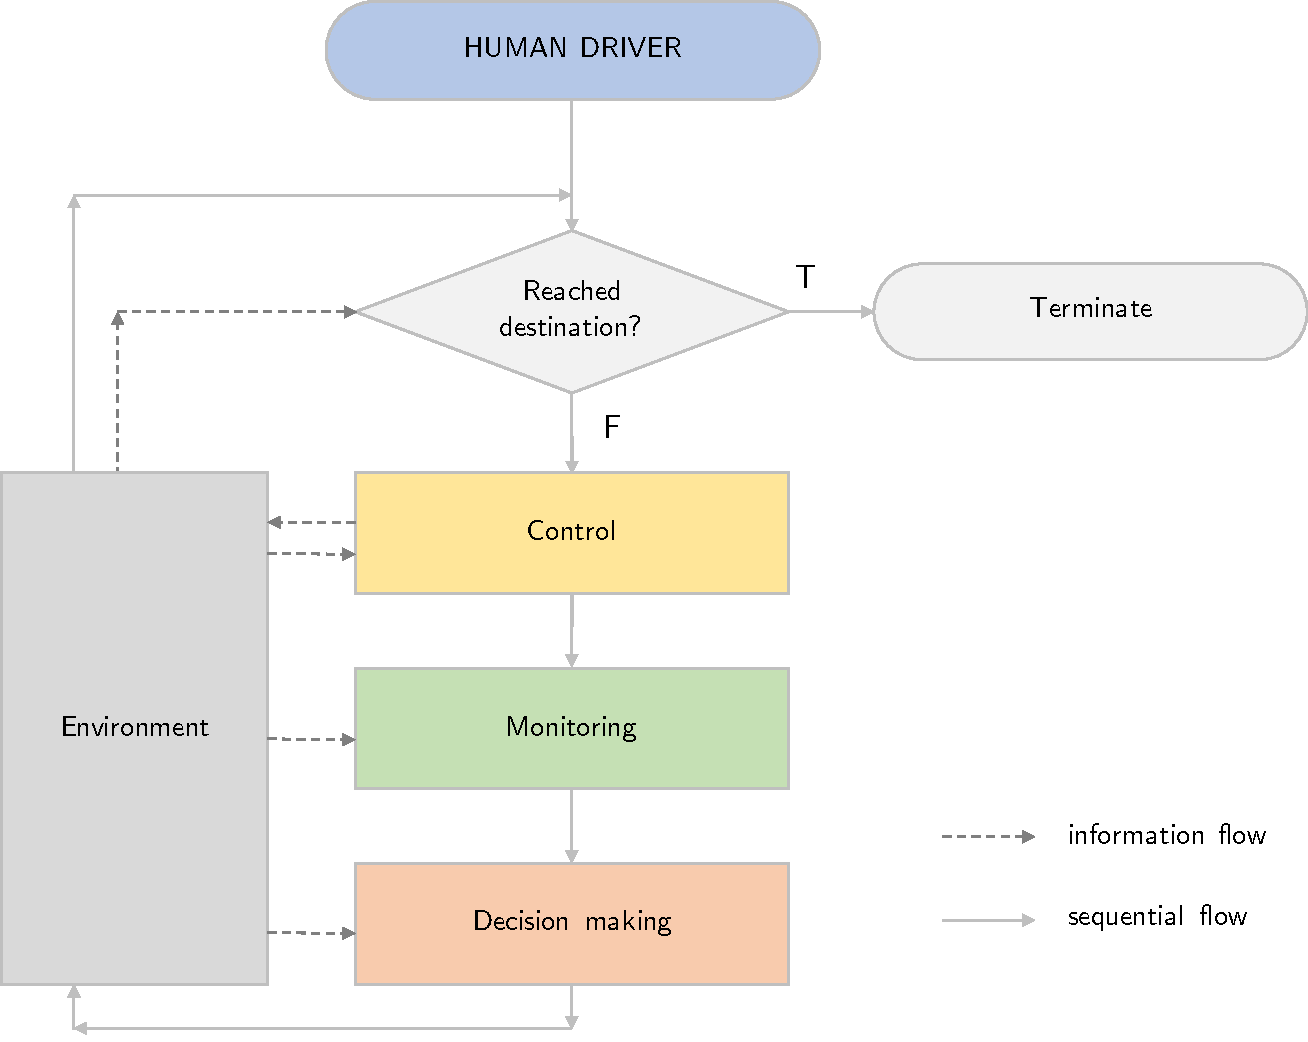
\includegraphics[width=0.85\textwidth]{matlab.pdf}
    \caption{Continuous Driver Model overview.}
    \label{fig:driver_model_overview}
\end{figure}

The monitoring module is implemented according to the flowchart presented in Figure~\ref{fig:monitor}, from the description given in \cite{salvucci_1}. The threshold for monitoring is set at $0.2$, as this is the value suggested in Salvucci in \cite{salvucci_1}. The output of this process corresponds to altering the global variable $a$ corresponding to the declarative memory cell composed of $k$ chunks. No specific value for $k$ is given by Salvucci in \cite{salvucci_1}, but it is taken to be 8 from \cite{lam}. The function \texttt{GET\_DISTANCE} is not described in depth due to the fact that it is trivial under the assumption stated in the previous paragraph.

The overall flowchart of the decision making module is shown in Figure~\ref{fig:dm}. The high level part is similar to the flowchart presented in Figure~\ref{fig:flowchart_dm}, with small differences related to the loading of variables and information from the different memories available. It is worth noticing that the control makes use of the function \texttt{LOOK\_VEHICLE} initially presented in the monitoring module to verify the presence of a vehicle in a relative position of a lane. The function \texttt{SET\_LANE\_FOLLOWING} is also omitted due to the trivial nature of this function under the assumptions made.

Finally, a flowchart for the control module is presented in Figure~\ref{fig:control}. This module is responsible for the calculation of $\Delta\varphi(t)$ and $\Delta\psi(t)$ and the update of the position. Given these two values, the position is updated following discrete laws of motion applied to rigid objects:

\begin{equation}
\begin{aligned}
	& \mathbf{v}(t) = \mathbf{v}(t-1) + \mathbf{a}(t)\Delta t\\
	& \mathbf{x}(t) = \mathbf{x}(t-1) + \mathbf{v}(t-1)\Delta t + \frac{1}{2}  \mathbf{a}(t)\Delta t^2 \\
	& t = t + \Delta t
\end{aligned}
\end{equation}

where $\mathbf{x}(t) = (x(t), y(t))$, $\mathbf{v}(t) = (v_x(t), v_y(t))$, and $\mathbf{a}(t) = (a_x(t), a_y(t))$, with:

\begin{equation}
\begin{aligned}
	a_x(t) & = \Delta\psi(t) \\
	a_y(t) & = \sin(\Delta\varphi(t))
\end{aligned}
\end{equation}

\begin{figure}
\centering
\begin{subfigure}{1\textwidth}
  \centering
  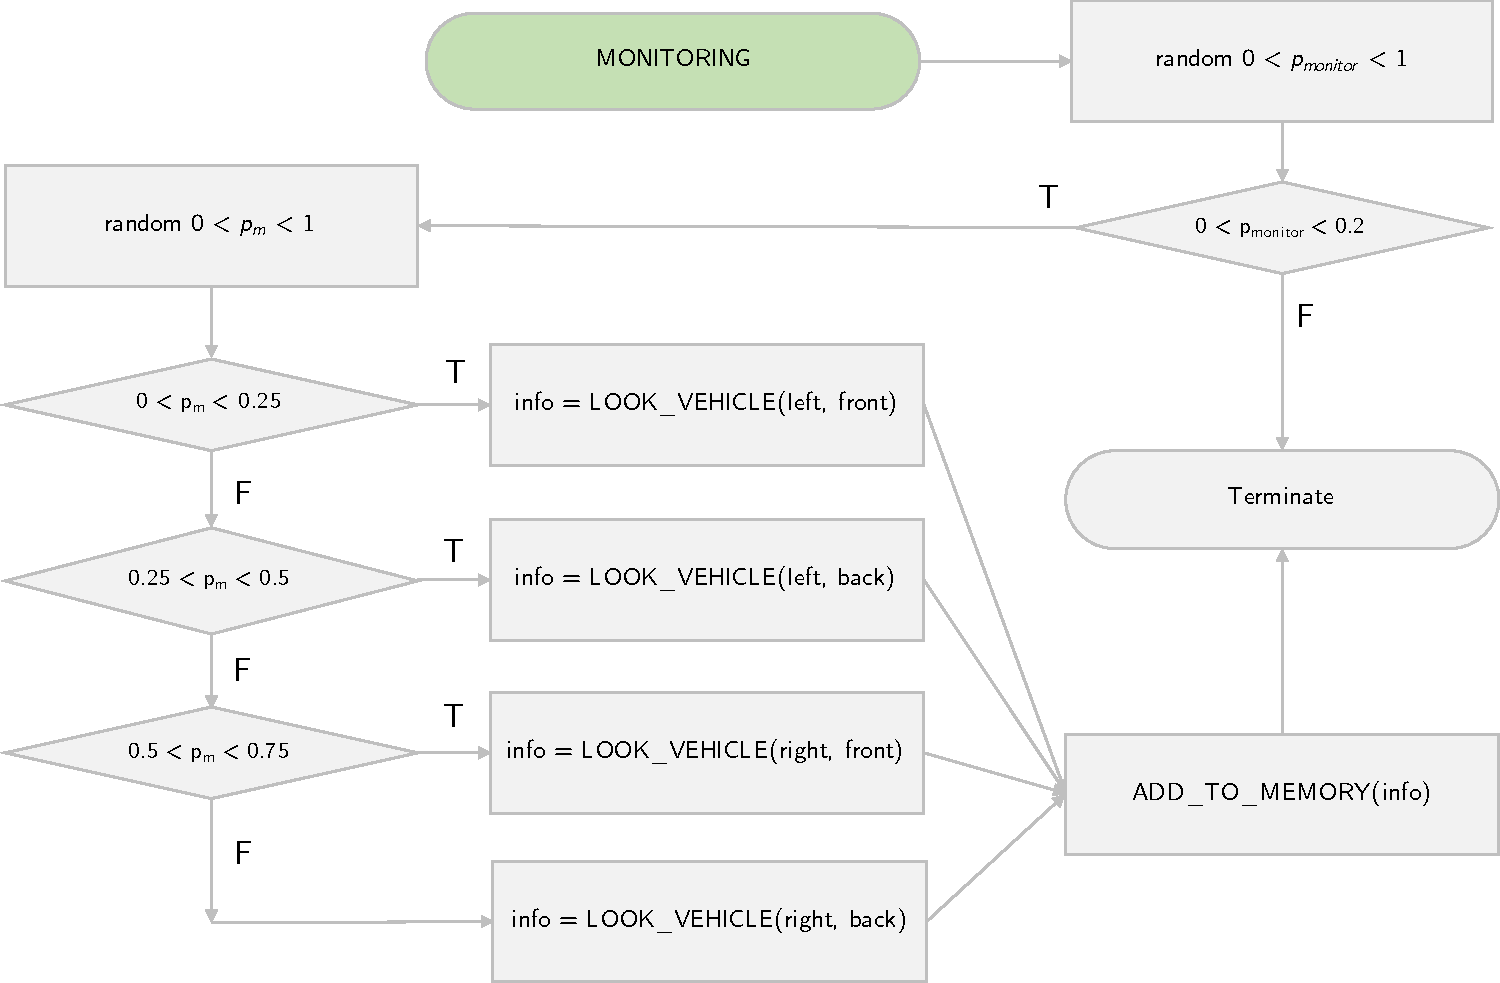
\includegraphics[width=1\textwidth]{monitor_1.pdf}
\end{subfigure}\\ \vspace{2em}
\begin{subfigure}{1\textwidth}
  \centering
  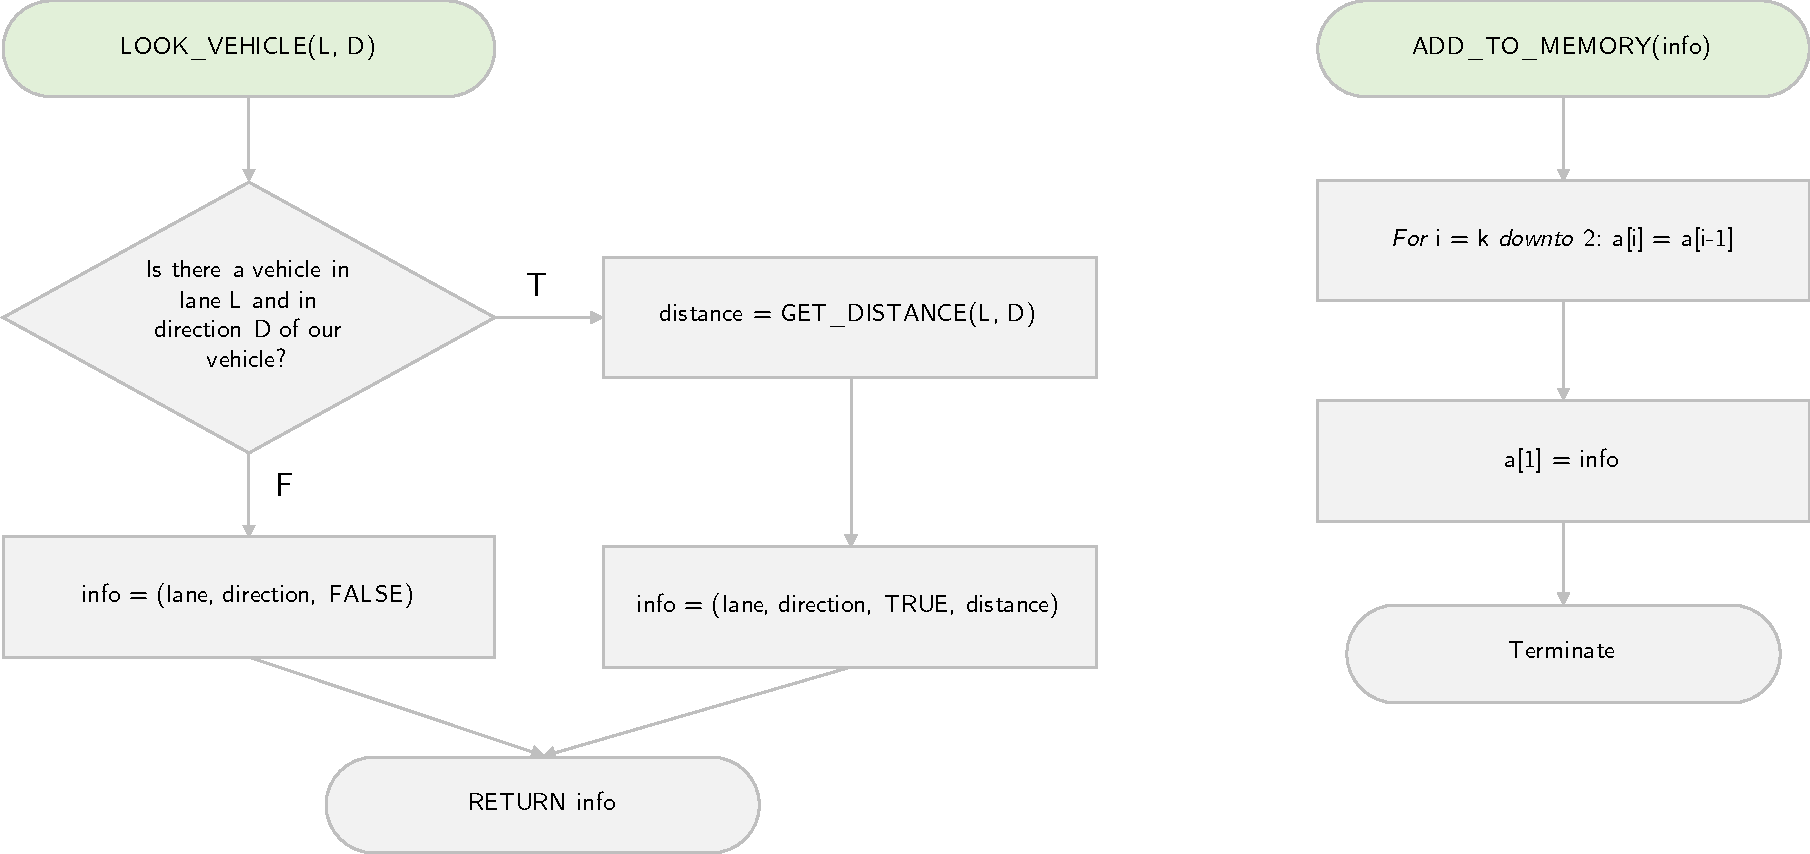
\includegraphics[width=1\linewidth]{monitor_2.pdf}
\end{subfigure} \vspace{2em}
\caption{Flowchart of the Monitoring module.}
\label{fig:monitor}
\end{figure}

\begin{figure}
\centering
\begin{subfigure}{1\textwidth}
  \centering
  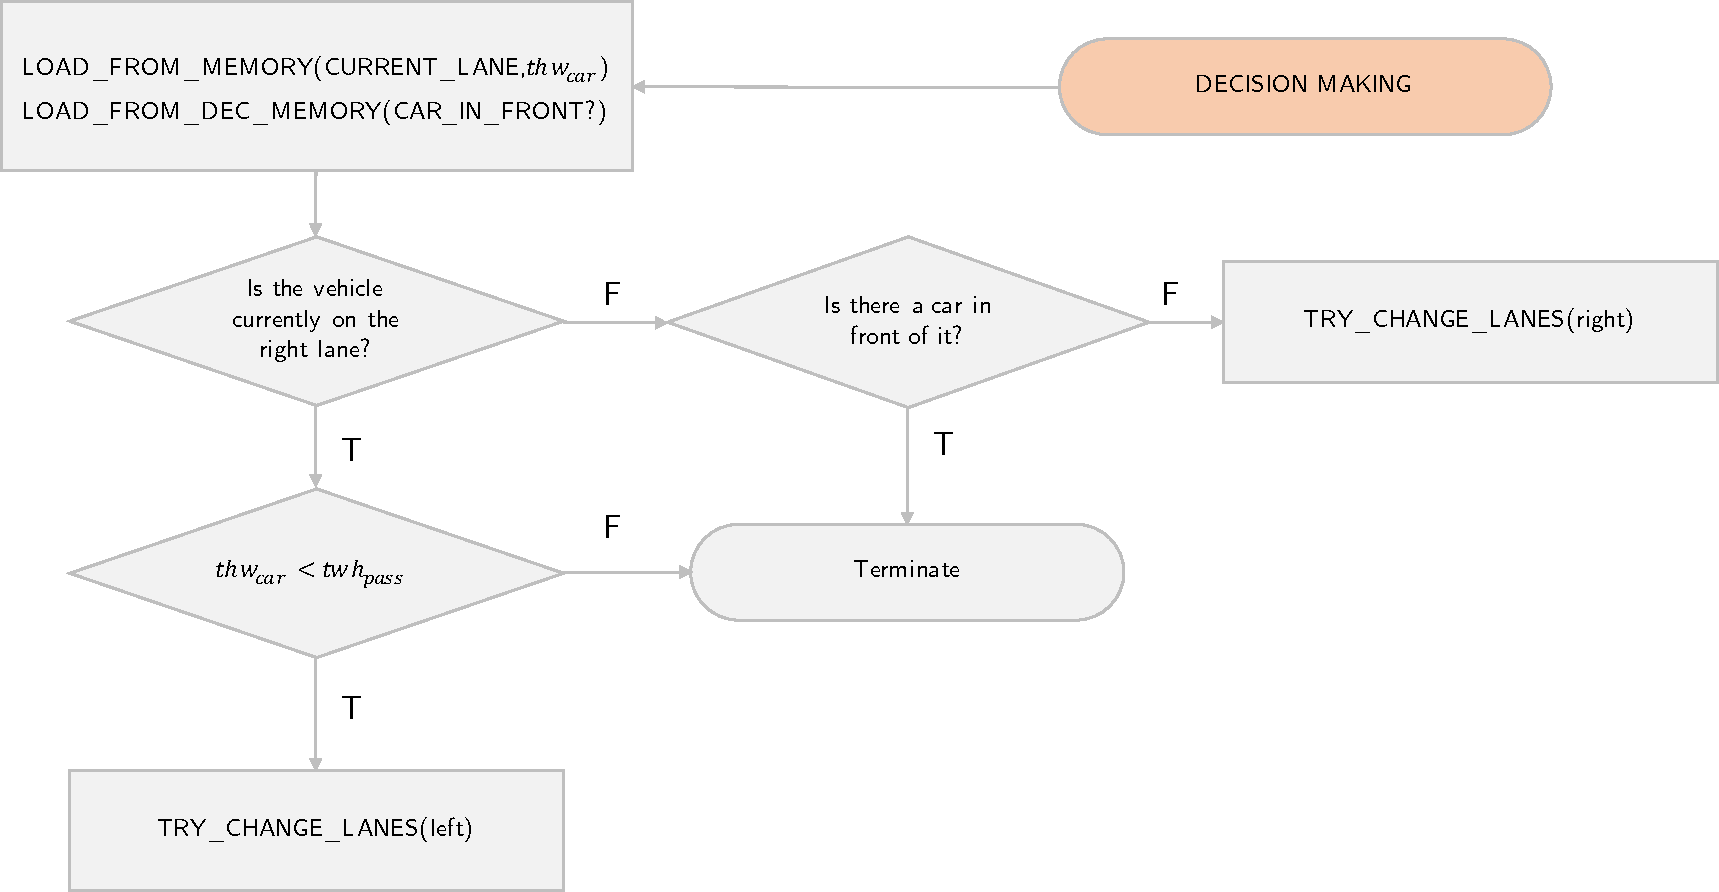
\includegraphics[width=1\textwidth]{dm_1.pdf}
\end{subfigure}\\ \vspace{2em}
\begin{subfigure}{1\textwidth}
  \centering
  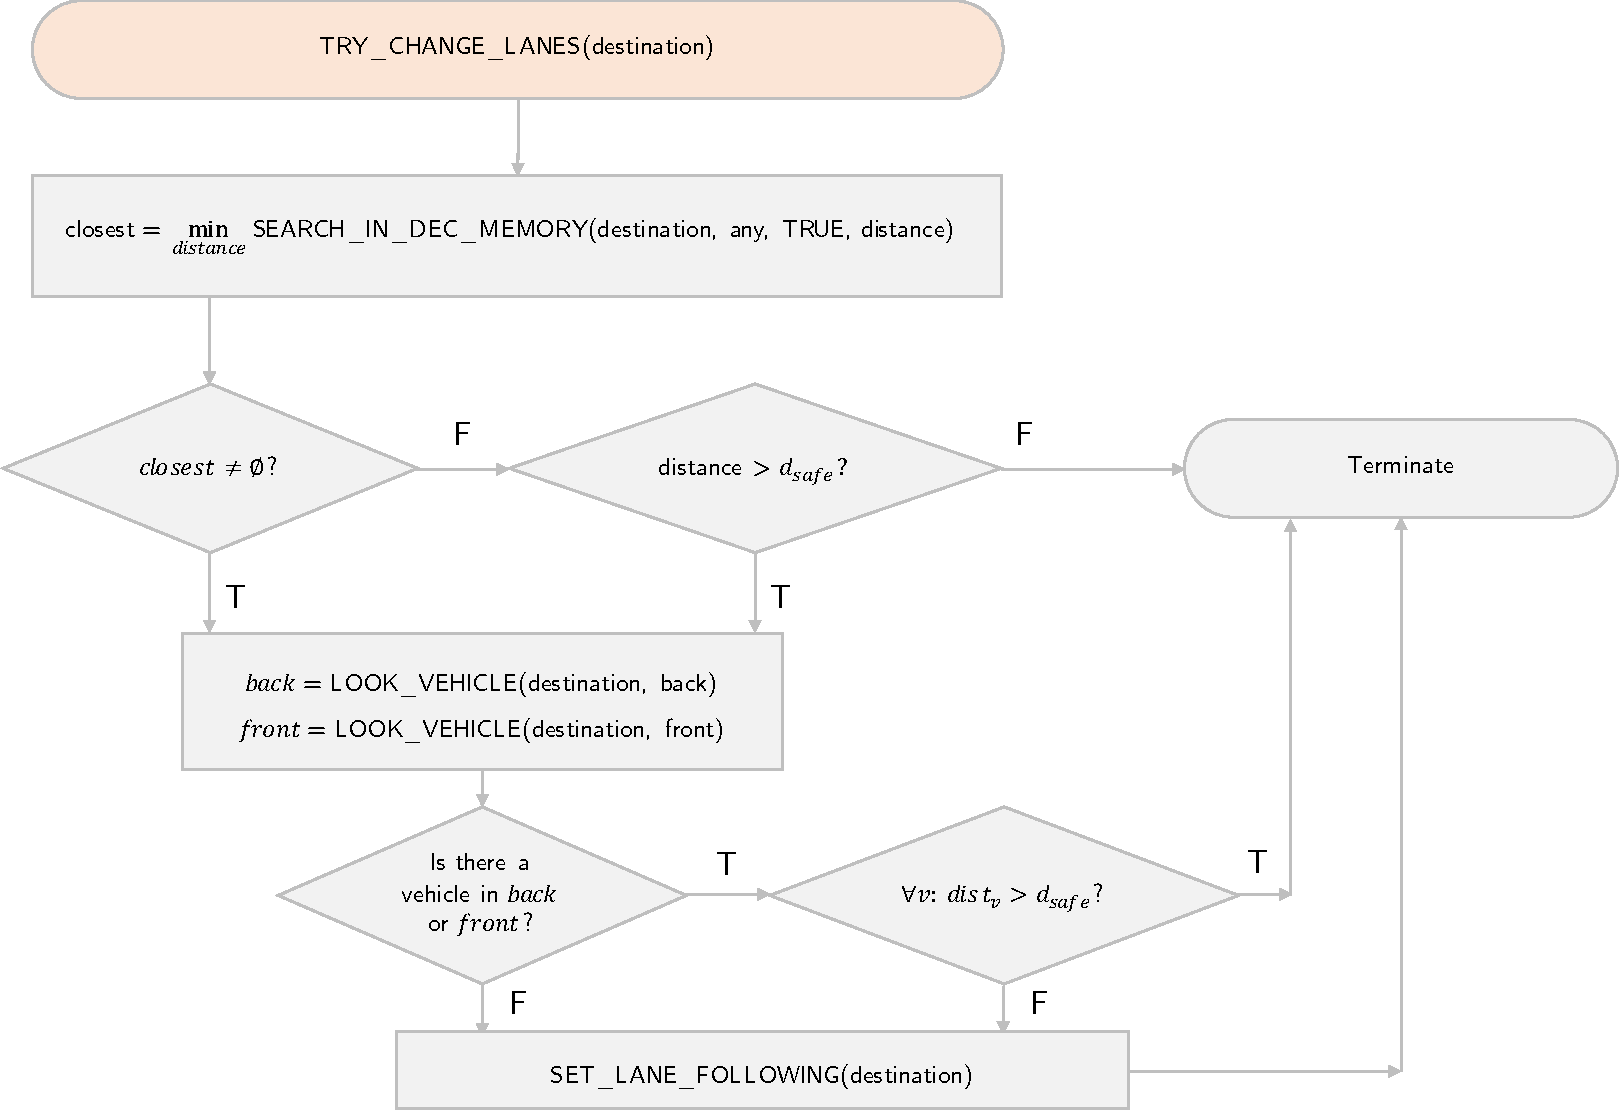
\includegraphics[width=1\linewidth]{dm_2.pdf}
\end{subfigure} \vspace{2em}
\caption{Flowchart of the Decision Making module.}
\label{fig:dm}
\end{figure}

\begin{figure}
\centering
\begin{subfigure}{1\textwidth}
  \centering
  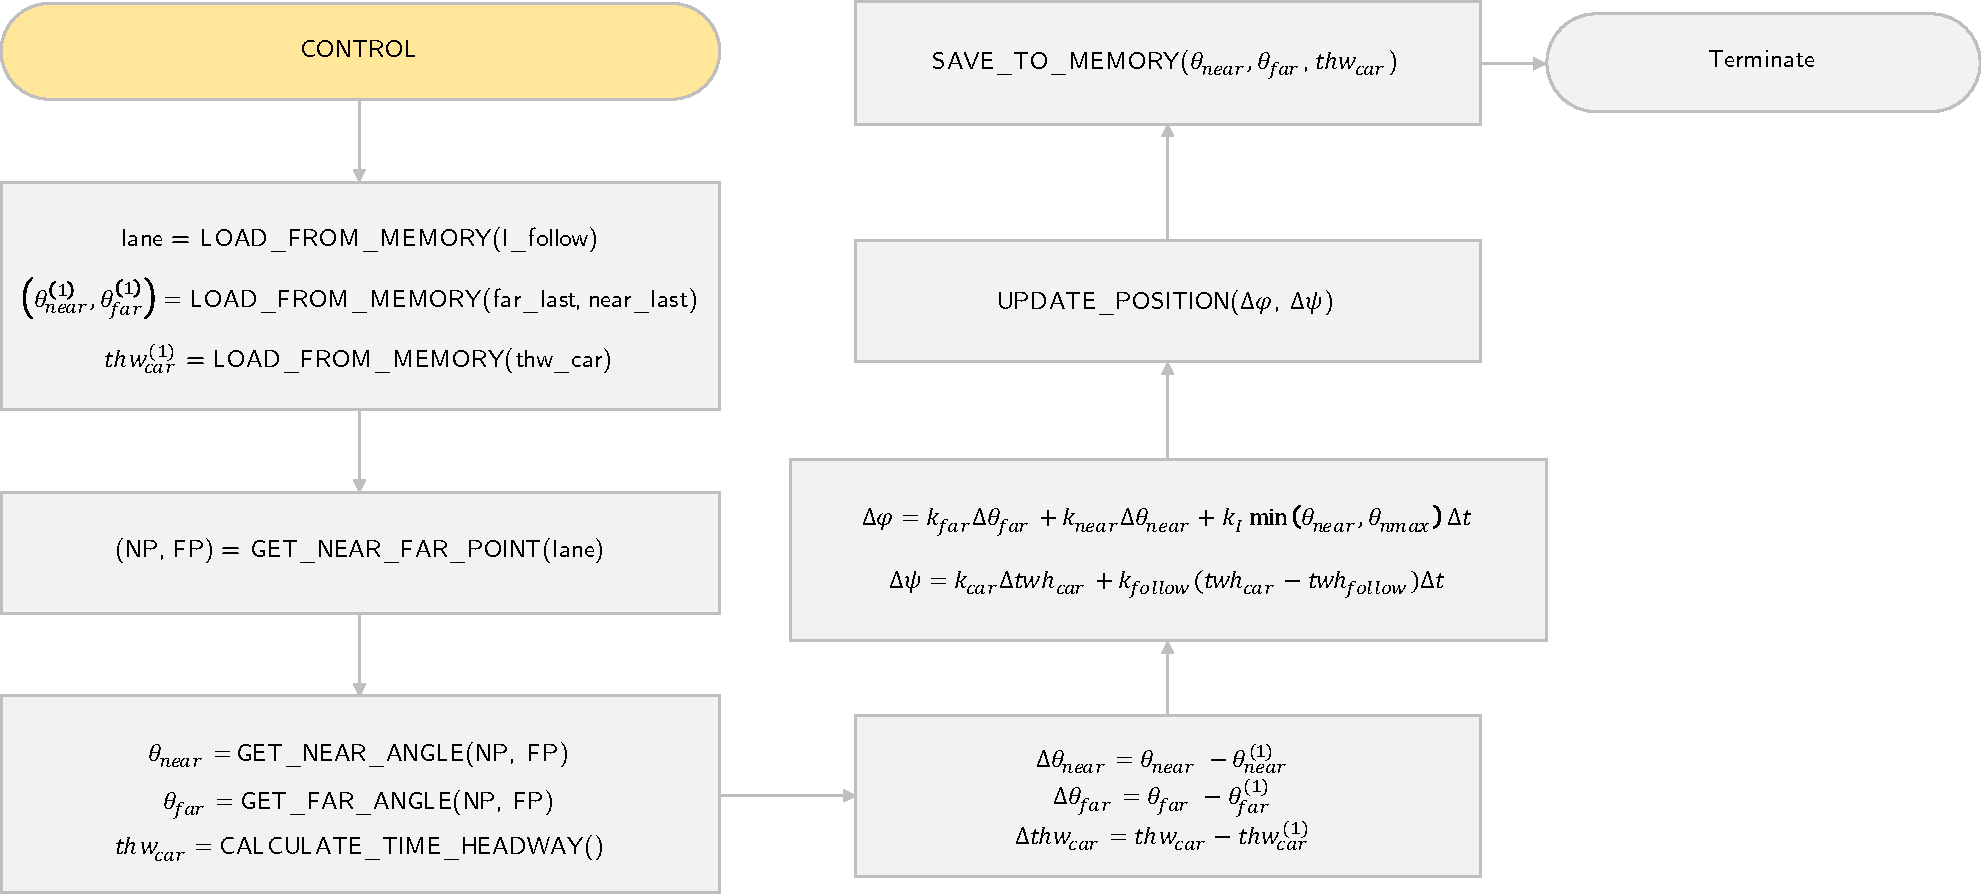
\includegraphics[width=1\textwidth]{control_1.pdf}
\end{subfigure}\\ \vspace{2em}
\begin{subfigure}{1\textwidth}
  \centering
  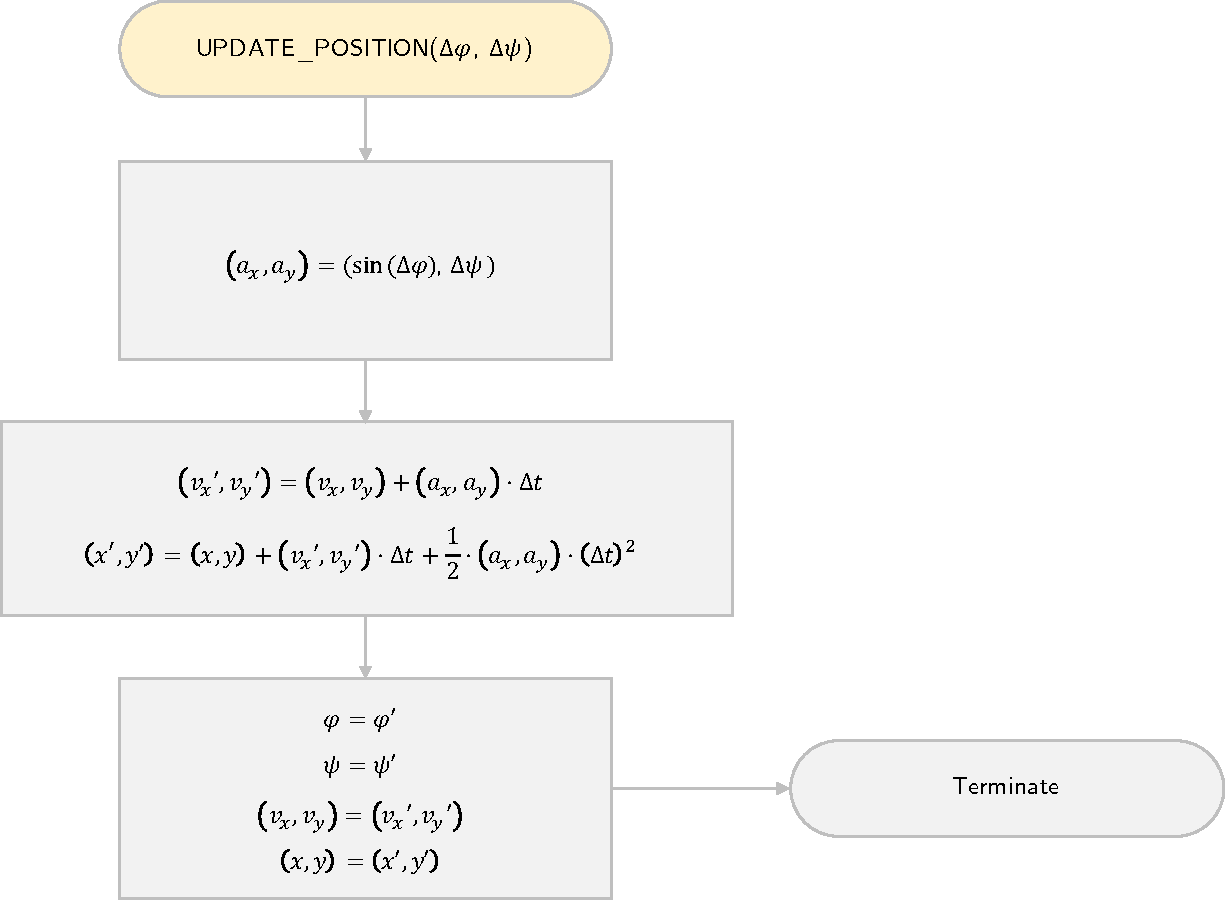
\includegraphics[width=0.7\linewidth]{control_2.pdf}
\end{subfigure} \vspace{2em}
\caption{Flowchart of the Control module.}
\label{fig:control}
\end{figure}

In this case, as Salvucci mentions in \cite{salvucci_1}, $\Delta t = 0.5s$. It is also assumed that the vehicle does not speed, and therefore, $v_x \in [15, 34]\text{ }m/s$ (between $50km/h$ and $120km/h$ - typical limits in highway speeds).

\section{Model Abstraction}

Lorem ipsum dolor sit amet, consectetur adipiscing elit. Pellentesque accumsan magna eu metus congue, vitae tristique enim commodo. Aliquam consectetur porttitor nisl, eget pulvinar quam venenatis eget. Aliquam erat volutpat. Nullam at ipsum at felis tincidunt consequat non sed mi. Morbi placerat iaculis dapibus. Aliquam non risus ac urna interdum pretium. Donec maximus, massa vitae suscipit congue, ligula purus sagittis magna, vitae interdum enim dui sed felis. Curabitur mollis eleifend diam a varius. Vivamus eu porttitor lorem. Mauris sagittis ultrices ligula, a euismod mi efficitur a. Aenean molestie sapien a nibh suscipit, nec venenatis urna varius. Sed eu ex id lacus tincidunt ultricies. Aenean quam massa, dignissim ac suscipit posuere, varius sit amet turpis. Nunc semper turpis ullamcorper elit venenatis, in molestie nulla fermentum.

\subsection{Non-Probabilistic Control Module}

Lorem ipsum dolor sit amet, consectetur adipiscing elit. Pellentesque accumsan magna eu metus congue, vitae tristique enim commodo. Aliquam consectetur porttitor nisl, eget pulvinar quam venenatis eget. Aliquam erat volutpat. Nullam at ipsum at felis tincidunt consequat non sed mi. Morbi placerat iaculis dapibus. Aliquam non risus ac urna interdum pretium. Donec maximus, massa vitae suscipit congue, ligula purus sagittis magna, vitae interdum enim dui sed felis. Curabitur mollis eleifend diam a varius. Vivamus eu porttitor lorem. Mauris sagittis ultrices ligula, a euismod mi efficitur a. Aenean molestie sapien a nibh suscipit, nec venenatis urna varius. Sed eu ex id lacus tincidunt ultricies. Aenean quam massa, dignissim ac suscipit posuere, varius sit amet turpis. Nunc semper turpis ullamcorper elit venenatis, in molestie nulla fermentum.

\subsection{Decision Making and Monitoring Module}

Lorem ipsum dolor sit amet, consectetur adipiscing elit. Pellentesque accumsan magna eu metus congue, vitae tristique enim commodo. Aliquam consectetur porttitor nisl, eget pulvinar quam venenatis eget. Aliquam erat volutpat. Nullam at ipsum at felis tincidunt consequat non sed mi. Morbi placerat iaculis dapibus. Aliquam non risus ac urna interdum pretium. Donec maximus, massa vitae suscipit congue, ligula purus sagittis magna, vitae interdum enim dui sed felis. Curabitur mollis eleifend diam a varius. Vivamus eu porttitor lorem. Mauris sagittis ultrices ligula, a euismod mi efficitur a. Aenean molestie sapien a nibh suscipit, nec venenatis urna varius. Sed eu ex id lacus tincidunt ultricies. Aenean quam massa, dignissim ac suscipit posuere, varius sit amet turpis. Nunc semper turpis ullamcorper elit venenatis, in molestie nulla fermentum.

\subsection{Probabilistic Control Module}

Lorem ipsum dolor sit amet, consectetur adipiscing elit. Pellentesque accumsan magna eu metus congue, vitae tristique enim commodo. Aliquam consectetur porttitor nisl, eget pulvinar quam venenatis eget. Aliquam erat volutpat. Nullam at ipsum at felis tincidunt consequat non sed mi. Morbi placerat iaculis dapibus. Aliquam non risus ac urna interdum pretium. Donec maximus, massa vitae suscipit congue, ligula purus sagittis magna, vitae interdum enim dui sed felis. Curabitur mollis eleifend diam a varius. Vivamus eu porttitor lorem. Mauris sagittis ultrices ligula, a euismod mi efficitur a. Aenean molestie sapien a nibh suscipit, nec venenatis urna varius. Sed eu ex id lacus tincidunt ultricies. Aenean quam massa, dignissim ac suscipit posuere, varius sit amet turpis. Nunc semper turpis ullamcorper elit venenatis, in molestie nulla fermentum.


\section{Model Evaluation Metrics}

Lorem ipsum dolor sit amet, consectetur adipiscing elit. Pellentesque accumsan magna eu metus congue, vitae tristique enim commodo. Aliquam consectetur porttitor nisl, eget pulvinar quam venenatis eget. Aliquam erat volutpat. Nullam at ipsum at felis tincidunt consequat non sed mi. Morbi placerat iaculis dapibus. Aliquam non risus ac urna interdum pretium. Donec maximus, massa vitae suscipit congue, ligula purus sagittis magna, vitae interdum enim dui sed felis. Curabitur mollis eleifend diam a varius. Vivamus eu porttitor lorem. Mauris sagittis ultrices ligula, a euismod mi efficitur a. Aenean molestie sapien a nibh suscipit, nec venenatis urna varius. Sed eu ex id lacus tincidunt ultricies. Aenean quam massa, dignissim ac suscipit posuere, varius sit amet turpis. Nunc semper turpis ullamcorper elit venenatis, in molestie nulla fermentum.

\subsection{Completeness Property}

Lorem ipsum dolor sit amet, consectetur adipiscing elit. Pellentesque accumsan magna eu metus congue, vitae tristique enim commodo. Aliquam consectetur porttitor nisl, eget pulvinar quam venenatis eget. Aliquam erat volutpat. Nullam at ipsum at felis tincidunt consequat non sed mi. Morbi placerat iaculis dapibus. Aliquam non risus ac urna interdum pretium. Donec maximus, massa vitae suscipit congue, ligula purus sagittis magna, vitae interdum enim dui sed felis. Curabitur mollis eleifend diam a varius. Vivamus eu porttitor lorem. Mauris sagittis ultrices ligula, a euismod mi efficitur a. Aenean molestie sapien a nibh suscipit, nec venenatis urna varius. Sed eu ex id lacus tincidunt ultricies. Aenean quam massa, dignissim ac suscipit posuere, varius sit amet turpis. Nunc semper turpis ullamcorper elit venenatis, in molestie nulla fermentum.

\subsection{Safety Property}

Lorem ipsum dolor sit amet, consectetur adipiscing elit. Pellentesque accumsan magna eu metus congue, vitae tristique enim commodo. Aliquam consectetur porttitor nisl, eget pulvinar quam venenatis eget. Aliquam erat volutpat. Nullam at ipsum at felis tincidunt consequat non sed mi. Morbi placerat iaculis dapibus. Aliquam non risus ac urna interdum pretium. Donec maximus, massa vitae suscipit congue, ligula purus sagittis magna, vitae interdum enim dui sed felis. Curabitur mollis eleifend diam a varius. Vivamus eu porttitor lorem. Mauris sagittis ultrices ligula, a euismod mi efficitur a. Aenean molestie sapien a nibh suscipit, nec venenatis urna varius. Sed eu ex id lacus tincidunt ultricies. Aenean quam massa, dignissim ac suscipit posuere, varius sit amet turpis. Nunc semper turpis ullamcorper elit venenatis, in molestie nulla fermentum.

\subsection{Liveness Properties}

Lorem ipsum dolor sit amet, consectetur adipiscing elit. Pellentesque accumsan magna eu metus congue, vitae tristique enim commodo. Aliquam consectetur porttitor nisl, eget pulvinar quam venenatis eget. Aliquam erat volutpat. Nullam at ipsum at felis tincidunt consequat non sed mi. Morbi placerat iaculis dapibus. Aliquam non risus ac urna interdum pretium. Donec maximus, massa vitae suscipit congue, ligula purus sagittis magna, vitae interdum enim dui sed felis. Curabitur mollis eleifend diam a varius. Vivamus eu porttitor lorem. Mauris sagittis ultrices ligula, a euismod mi efficitur a. Aenean molestie sapien a nibh suscipit, nec venenatis urna varius. Sed eu ex id lacus tincidunt ultricies. Aenean quam massa, dignissim ac suscipit posuere, varius sit amet turpis. Nunc semper turpis ullamcorper elit venenatis, in molestie nulla fermentum.

\section{Simulation of Paths in the Model}
\label{sec:simulator}

Lorem ipsum dolor sit amet, consectetur adipiscing elit. Pellentesque accumsan magna eu metus congue, vitae tristique enim commodo. Aliquam consectetur porttitor nisl, eget pulvinar quam venenatis eget. Aliquam erat volutpat. Nullam at ipsum at felis tincidunt consequat non sed mi. Morbi placerat iaculis dapibus. Aliquam non risus ac urna interdum pretium. Donec maximus, massa vitae suscipit congue, ligula purus sagittis magna, vitae interdum enim dui sed felis. Curabitur mollis eleifend diam a varius. Vivamus eu porttitor lorem. Mauris sagittis ultrices ligula, a euismod mi efficitur a. Aenean molestie sapien a nibh suscipit, nec venenatis urna varius. Sed eu ex id lacus tincidunt ultricies. Aenean quam massa, dignissim ac suscipit posuere, varius sit amet turpis. Nunc semper turpis ullamcorper elit venenatis, in molestie nulla fermentum.
